This section will cover the testing phase of the projects, and describe how tests were performed. The focus of the tests is on the lexical analysis and the compiler.\todo{Morten:Med compiler, menes der så kodegenerering?}

\section{Testing Method}
There are a wide range of methods available for testing software. They can however be broken into two main categories named white- and black box testing. Black box testing can be interpreted as the program being a black box with unkown content. What is known is that given some input to the box, an appropriate output is expected. In other terms the focus is not on how it works, rather that it just works. With white box testing however, the focus is as much on how the output is generated from the input.\\

Both methods have their own advantages, briefly described below:
\begin{itemize}
\item[] \textbf{Black box} It is not necessary to have any knowledge of the code. To test the software, the tester only needs to know how to pass the input parameter and what to expect as output. This also makes it faster to run and evaluate the tests, since the MORTEN-ADDITION: technical details do not have to be accounted for.\todo{Morten: Der manglede en halv sætning her. :p }
\item[] \textbf{White box} With white-box testing, testing the the code itself, it is possible to use these tests to optimize the code. It is however also more demanding, as the tests require knowledge of the code in order to be able to design the tests. 
\end{itemize}

\subsection*{Syntax}
\begin{table}[thp]\scriptsize
\centering
\begin{tabular}{|l|l|c|}
\multicolumn{1}{c}{Test case} &
\multicolumn{1}{c}{Result} &
\multicolumn{1}{c}{} \\
\hline
{\begin{lstlisting}[numbers=none,frame=none,resetmargins=true]
void setup() do
end
\end{lstlisting}} & 
{\begin{lstlisting}[numbers=none,frame=none,resetmargins=true]
void setup(){
}
\end{lstlisting}} &
\checkmark\\
  \hline
{\begin{lstlisting}[numbers=none,frame=none,resetmargins=true]
instantiate LiquidCrystal lcd(12,11,5);
CALL lcd.print("Hello World"); 
\end{lstlisting}} & 
{\begin{lstlisting}[numbers=none,frame=none,resetmargins=true]
LiquidCrystal lcd(12,11,5);
lcd.print("Hello World");
\end{lstlisting}} &
\checkmark\\
\hline
{\begin{lstlisting}[numbers=none,frame=none,resetmargins=true]
if(true)do
	x = 1;
end
else do
	x = 2;
end 
\end{lstlisting}} & 
{\begin{lstlisting}[numbers=none,frame=none,resetmargins=true]
if(true){
	x = 1;
}
else {
	x = 2;
} 
\end{lstlisting}} &
\checkmark\\
\hline
\end{tabular}
\caption{Examples of test cases}
\label{tab:test}
\end{table}

The test case shown in table \ref{tab:test} is just an example of the cases run during the development of the compiler. More complex cases were tested, but have been omitted due to readability. Examples of these test cases are the complete code examples found in chapter \ref{sec:code_examples}, code example \ref{lst:syntax1} and \ref{lst:syntax2}\\

The tests have been conducted repeatedly through the process every time a new feature or functionality has been implemented, to help make sure that the new version works as intended, and that it does not break other parts unintentionally.

\subsection*{Error messages}
If the compiler encounters any errors during compilation of a program, appropriate error messages are displayed to help guide the user in the right direction, when trying to locate the cause of errors.

It is important to point out that for some of the test cases, the purpose of the test is to fail. This is in order to make sure that error messages are only shown when the error actually occurs. This means that if the test fail (No errors displayed), the program works as intended and the test is a success.\\
\begin{table}[thp]\scriptsize
\raggedright
\begin{tabular}{|l|m{10cm}|c|}
\multicolumn{1}{c}{Test case} &
\multicolumn{1}{c}{Expected result} &
\multicolumn{1}{c}{} \\
\hline
{\begin{lstlisting}[numbers=none,frame=none,resetmargins=true]
boolean x = 1 + 3; 
\end{lstlisting}} &
{\begin{lstlisting}[numbers=none,frame=none,resetmargins=true,language={}]
_errorMessage = "A variable of type boolean has to have an integer (1,0) or identifier (true, false) as value.";
\end{lstlisting}} &
\checkmark\\
\hline
{\begin{lstlisting}[numbers=none,frame=none,resetmargins=true]
int x = 2;
float y = 5.2;
int z = x + y; 
\end{lstlisting}} &
{\begin{lstlisting}[numbers=none,frame=none,resetmargins=true,language={}]
_errorMessage = "Trying to add Float to Integer, this result in loss of precision.";
\end{lstlisting}} &
\checkmark\\
\hline
{\begin{lstlisting}[numbers=none,frame=none,resetmargins=true]
void loop() do
 float b =  .10 + 1.12312;
 int h = 10/1 //Missing ;
 string he = "hello";
end
\end{lstlisting}} &
{\begin{lstlisting}[numbers=none,frame=none,resetmargins=true,language={}]
Exception in thread "main" ParseException: Encountered " "string" "string "" at line 3, column 9.
\end{lstlisting}} &
\checkmark\\
\hline
{\begin{lstlisting}[numbers=none,frame=none,resetmargins=true]
boolean x = 1; 
\end{lstlisting}} &
{\begin{lstlisting}[numbers=none,frame=none,resetmargins=true,language={}]
_errorMessage = "A variable of type boolean has to have an integer (1,0) or identifier (true, false) as value.";
\end{lstlisting}} &
$\bigotimes$\\
\hline
{\begin{lstlisting}[numbers=none,frame=none,resetmargins=true]
float x = 2;
float y = 5.2;
float z = x + y; 
\end{lstlisting}} &
{\begin{lstlisting}[numbers=none,frame=none,resetmargins=true,language={}]
_errorMessage = "Trying to add Float to Integer, this result in loss of precision.";
\end{lstlisting}} &
$\bigotimes$\\
\hline
{\begin{lstlisting}[numbers=none,frame=none,resetmargins=true]
void loop() do
 float b =  .10 + 1.12312;
 int h = 10/1;
 string he = "hello";
end
\end{lstlisting}} &
{\begin{lstlisting}[numbers=none,frame=none,resetmargins=true,language={}]
Exception in thread "main" ParseException: Encountered " "string" "string "" at line 3, column 9.
\end{lstlisting}} &
$\bigotimes$\\
\hline
\end{tabular}
\caption{Different examples of error messages}
\label{tab:type_test}
\end{table}

The last 3 test cases in table \ref{tab:type_test} are all meant to fail, to make sure the error messages do not display when there are no errors.

\section{Functionality}
To verify that the compiled program can actually run on Arduino, two test programs are used to test the compiled program. These are the code examples from chapter \ref{analysis:syntax-examples} and the corresponding Arduino programs can be found in appendix \ref{app:code}\pagebreak
\subsection*{Hello World}
The first piece of code from example \ref{lst:syntax1} prints ''Hello, world'' and displays it for 2 seconds before continuing with the rest of the program.
\begin{figure}[h]
\begin{lstlisting}[caption=Hello World ,firstnumber=11, language={C++}, label=lst:snippet_1]
  call lcd.begin(8, 2);
  // Print a message to the LCD.
  call lcd.print("hello, world!");
  call delay(2000);
\end{lstlisting}
\caption{snippet from code example \ref{lst:syntax1}}
\end{figure}
\begin{figure}[h]
\centering
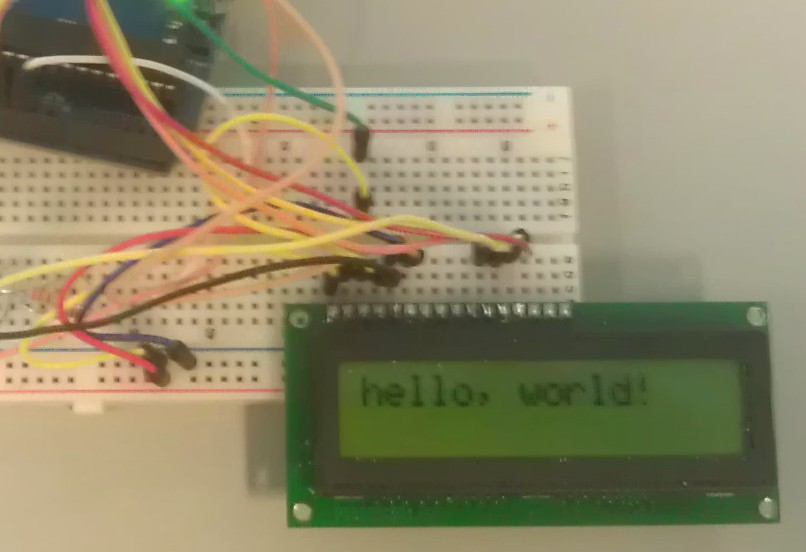
\includegraphics[width=8cm]{billeder/test_hello_1.jpg}
\caption{picture of the execution of code snippet \ref{lst:snippet_1}}
\end{figure}

The code snippet below is the main loop in the program. It runs continuously for as long as the Arduino is powered on and prints the uptime measured in seconds. Although this is a rather simple program, it does prove that the basic functionality of the compiler is working as intended.
\begin{figure}[h]
\begin{lstlisting}[caption=Hello World ,firstnumber=17, language={C++},label=lst:snippet_2]
void loop() do
  call lcd.clear();

  // print the number of seconds since reset:
  int runTime = millis();
  int time = runTime/1000;
  call lcd.print(time);


  call delay(1000);
end
\end{lstlisting}
\caption{snippet from code example \ref{lst:syntax1}}
\end{figure}
\begin{figure}[htb]
\centering
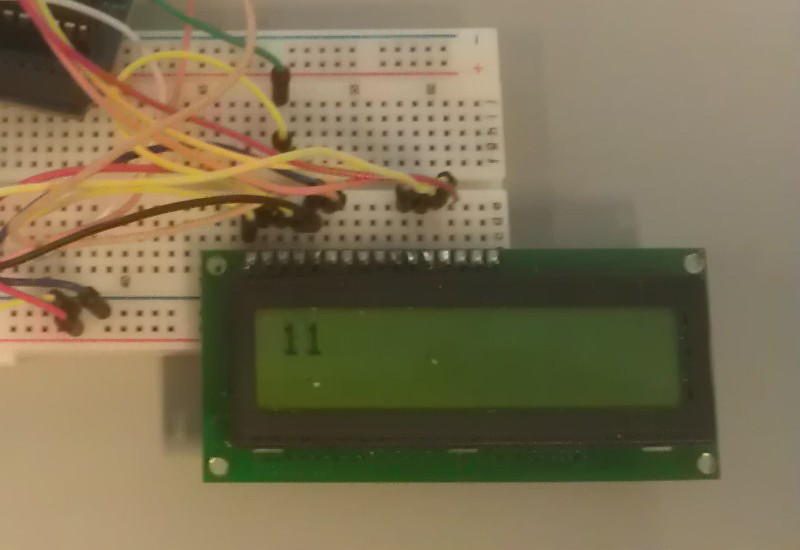
\includegraphics[width=8cm]{billeder/test_hello_2.jpg}
\caption{picture of the execution of code snippet \ref{lst:snippet_2}}
\end{figure}

During the tests a persistant error occured multiple times. While running a program, the screen would suddenly display seemingly random symbols as seen in figure \ref{fig:symbolerror}. The Arduino IDE offers easy monitoring of serial output from Arduino which makes it possible to monitor what is printed to the LCD display, by also sending it to a computer through a serial connection.
\begin{figure}[h]
\centering
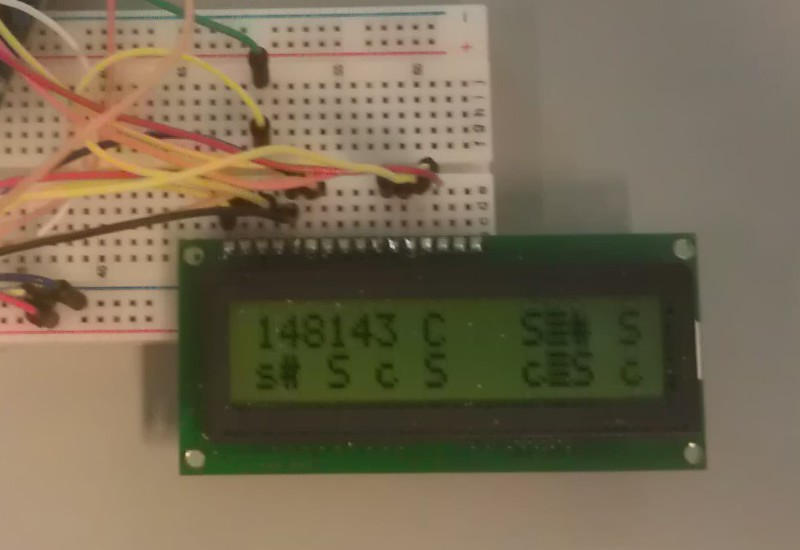
\includegraphics[width=8cm]{billeder/test_giberish.jpg}
\caption{Example of printing random symbols}
\label{fig:symbolerror}
\end{figure}

\begin{figure}[hbtp]
\centering
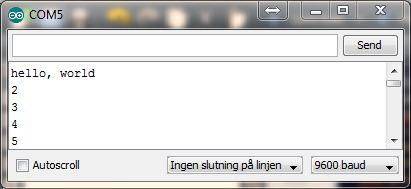
\includegraphics[width=8cm]{billeder/arduino_serial_output.JPG}
\caption{Print from Arduino IDE serial monitor showing the correct output}
\label{fig:serial}
\end{figure}

By adding a few lines of code to the Hello world code example \ref{lst:syntax1}, the addition of lines 2, 6, 12 and 14, in code example \ref{lst:serial} makes it possible to view the data printed to the LCD display, as seen in figure \ref{fig:serial}. This has made it possible to verify that the problem is not with the data itself. An attempt was made to write the programs directly for Arduino, not using the compiler for PH, but the same error still occurred. This increases the likelihood that the problem is caused by the hardware rather than the software. This could theoretically be due to limitations of the hardware but is very unlikely since the examples used are copies of official Arduino guides. It is more likely that the error is due to faulty hardware, whether that be the Arduino board or the LCD display. Unfortunately it was not possible to test the theory as we did not have access to replacement hardware.

\begin{figure}[h!]
\begin{lstlisting}[caption=Hello World with serial output, language={C++},label=lst:serial]
void setup() do
  call Serial.begin(9600);
  call lcd.begin(8, 2);

  // Print a message to the LCD.
  call lcd.print("hello, world!");
  call Serial.println("hello, world!");
  call delay(2000);
end

void loop() do
  call lcd.clear();

  // print the number of seconds since reset:
  int runTime = millis();
  int time = runTime/1000;
  call lcd.print(time);
  call Serial.println(time);
  call delay(1000);
end
\end{lstlisting}
\caption{Code example \ref{lst:syntax1} modified to allow for serial output}
\end{figure}

\subsection*{FooBar}
The program from code example \ref{lst:syntax2} prints a message based on a number count between 1 and 100. It is a rather simple program, but does make use of some of the more advanced features of PH. A snippet of the code running the counter can be seen in code example \ref{lst:foobar}
\begin{lstlisting}[caption=Hello World with serial output,firstnumber=26, language={C++},label=lst:foobar]
if(count % 3 EQUALS 0 AND count % 5 equals 0) do
      call lcd.print("Foo Bar"); 
end
elseif(count % 3 EQUALS 0) do
    call lcd.print("Foo");
end
elseif(count % 5 EQUALS 0) do
    call lcd.print("Bar");
end
else do
    call lcd.print(count);
end
\end{lstlisting}

The program running in the pictures below have been modified to show both the count and the message to make it easier to see that it is in fact working as intended.

\begin{table}[h]
\begin{tabular}{p{8,5cm}p{8,5cm}}
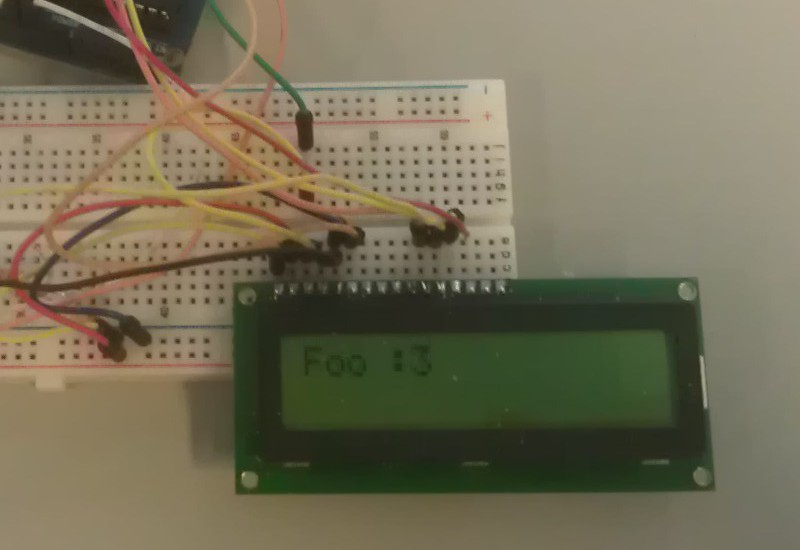
\includegraphics[width=8cm]{billeder/test_foobar_1.jpg}
Count = 3
 &
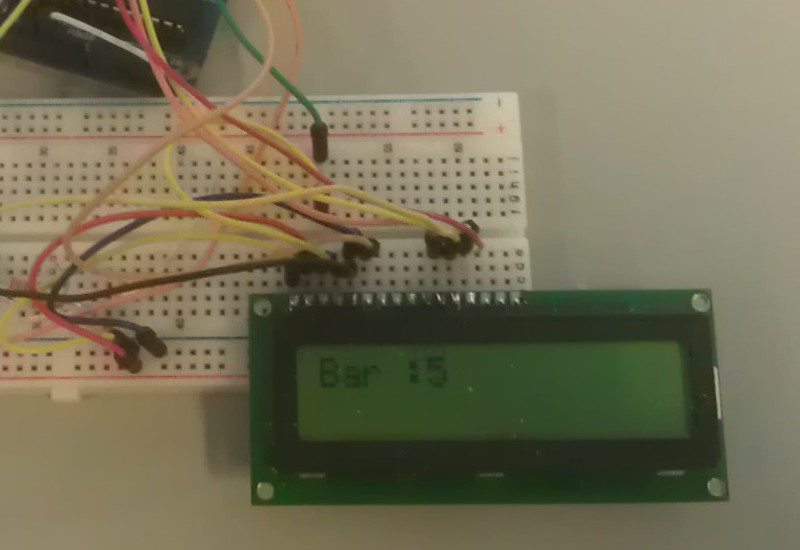
\includegraphics[width=8cm]{billeder/test_foobar_2.jpg}
Count = 5
\\ 
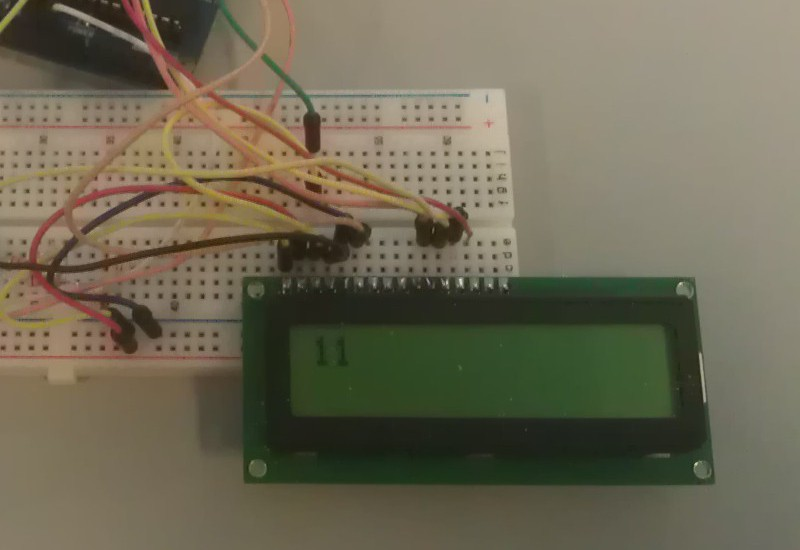
\includegraphics[width=8cm]{billeder/test_foobar_3.jpg}
Count = 11
 & 
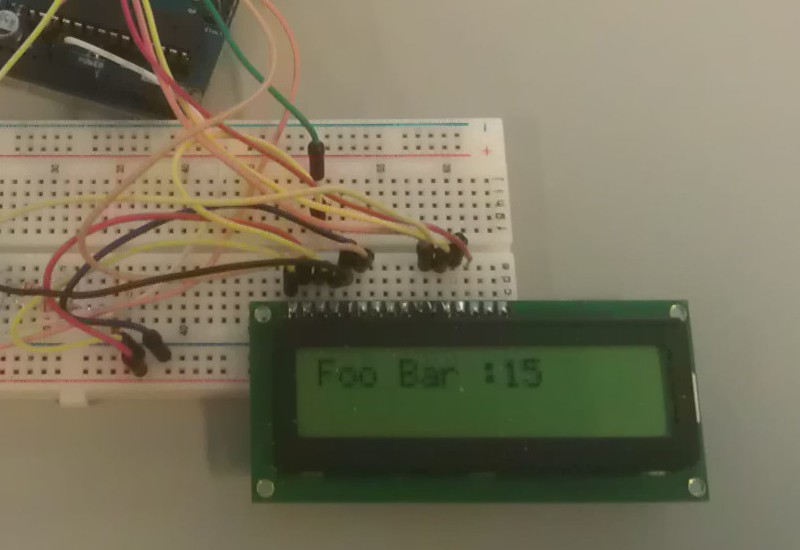
\includegraphics[width=8cm]{billeder/test_foobar_4.jpg}
Count = 15
 \\ 
\end{tabular} 
\caption{Examples of prints when running the Foobar program}
\end{table}

As expected, the Foobar program resulted in the same error, producing random symbols at the LCD display just as the Hello world test did. As with the the other test, none of the attempts to locate the error gave any results.